\subsection{Generación de señalamiento paso a paso}

Al ejecutar el RNA, primero detectará todos los \textit{netElements}, sus coordenadas iniciales y finales en la topología, y el sentido en el que fueron definidas. El resultado obtenido se muestra en el Cóodigo \ref{lst:EJ9_1}.

\begin{lstlisting}[language = {}, caption = Detección de \textit{netElements} por parte del RNA , label = {lst:EJ9_1}]
	###### Starting Railway Network Analyzer #####
	Reading .railML file
	Creating railML object
	Analysing railML object
	Analysing graph
	ne3 [9384, 0] [7584, 0] <<
	ne40 [1680, 0] [3796, 0] >>
	ne46 [3796, 0] [7584, 0] >>
	ne48 [4216, 420] [3796, 0] <<
	ne49 [4216, 420] [7164, 420] >>
	ne50 [7164, 420] [4216, 420] <<
	ne53 [7164, 420] [7584, 0] >>
	The network is connected
\end{lstlisting}

Por ejemplo, el \textit{netElement} ne50 inicia en la coordenada (7164;420) y finaliza en la coordenada (4216;420). El símbolo $<<$ indica que ne50 se encuentra definido de derecha a izquierda, ya que la componente x de la coordenada final es menor a la de la coordenada inicial, teniendo la misma componente y. Además, se puede comprobar que la lista obtenida en consistente con la Figura \ref{fig:EJ9_2}. Por ejemplo, ne48, ne49 y ne50 comparten la coordenada (4216;420), que coincide con la coordenada del cambio de vías Sw29.

A continuación, el RNA detectará la infraestructura ferroviaria, las curvas peligrosas y los puntos medios de los netElements que el RNA considera demasiado largos. El resultado de este proceso se puede visualizar en el Código \ref{lst:EJ9_2} y puede leerse también en el archivo Infrastructure.RNA.

\begin{lstlisting}[language = {}, caption = Detección de puntos críticos por parte del RNA , label = {lst:EJ9_2}]
	Analysing infrastructure --> Infrastructure.RNA
	Detecting Danger --> Safe_points.RNA
	ne3 has a RailJoint[J16] @ [7864, 0]
	ne3 has a RailJoint[J17] @ [8219, 0]
	ne3 has a RailJoint[J18] @ [8867, 0]
	ne3 has a Platform[Plat10] @ [8542, 0]
	ne40 has a RailJoint[J19] @ [3428, 0]
	ne40 has a RailJoint[J20] @ [2485, 0]
	ne40 has a RailJoint[J21] @ [2149, 0]
	ne40 has a Platform[Plat14] @ [2848, 0]
	ne46 has a RailJoint[J12] @ [4952, 0]
	ne46 has a RailJoint[J15] @ [6424, 0]
	ne46 has a Platform[Plat13] @ [5487, 0]
	ne46 has a LevelCrossing[Lc10] @ [5915, 0]
	ne49 has a RailJoint[J10] @ [4952, 870]
	ne49 has a RailJoint[J13] @ [6424, 870]
	ne49 has a Platform[Plat11] @ [5487, -870]
	ne49 has a LevelCrossing[Lc11] @ [6006, -870]
	ne49 has a Curve(3 lines) @ [[4666, 870], [6714, 870]]
	ne50 has a RailJoint[J11] @ [4952, 420]
	ne50 has a RailJoint[J14] @ [6424, 420]
	ne50 has a Platform[Plat12] @ [5487, -420]
	ne50 has a LevelCrossing[Lc09] @ [6096, -420]
\end{lstlisting}

Una vez que el RNA detectó cada punto crítico de la red ferroviaria, procede a generar el señalamiento. El orden de generación no es importante, pero para poder describirlo de forma consistente se iniciará generando el señalamiento para proteger los finales de vías, las junturas entre rieles, las plataformas, los cruces de vía y los cambios de vías. Luego se procederá a mostrar el señalamiento pre y post simplificación. Las señales generadas para proteger los finales de vías relativos y absolutos son ilustradas en la Figura \ref{fig:EJ9_3}.

\begin{figure}[H]
	\centering
	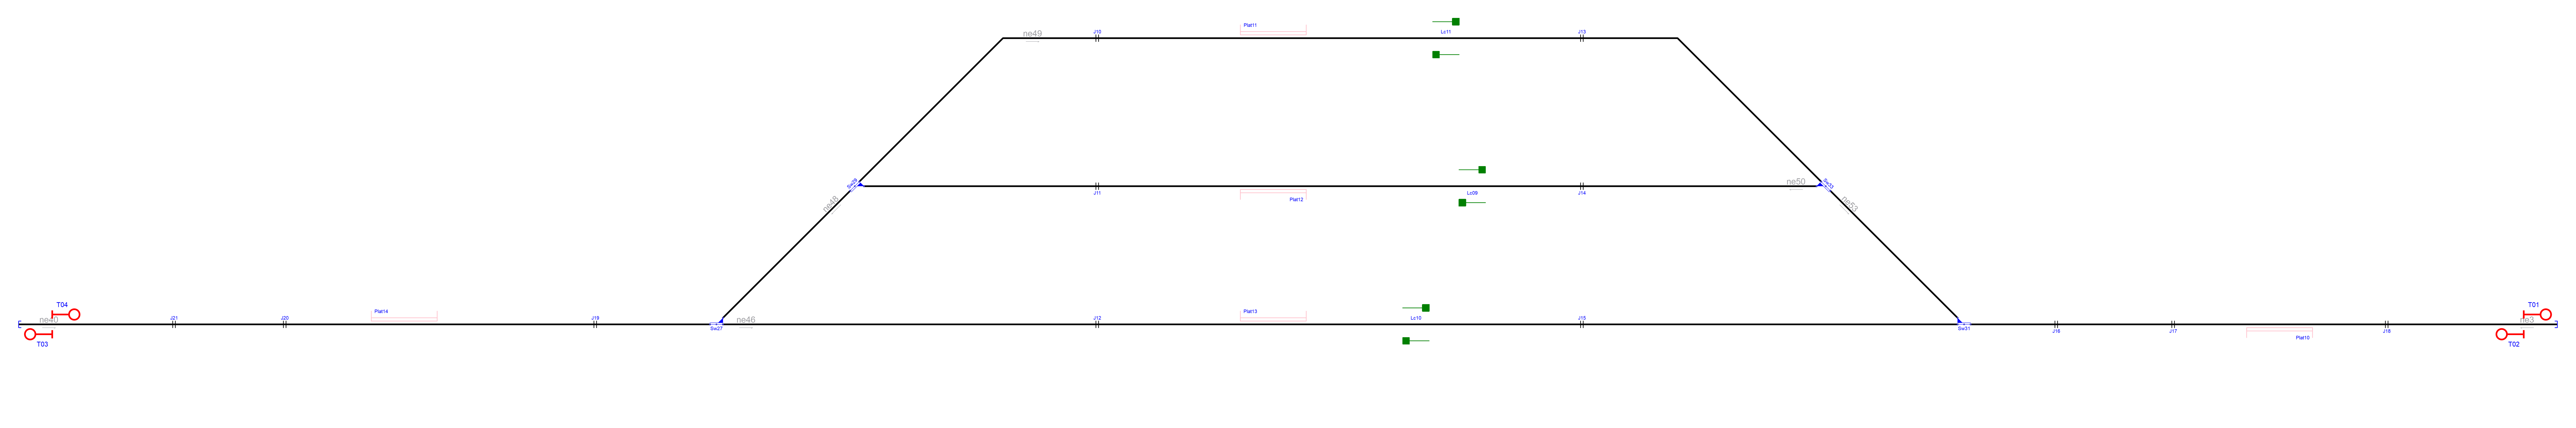
\includegraphics[width=1\textwidth]{resultados-obtenidos/ejemplo9/images/9_step1.png}
	\centering\caption{Señalamiento generado por el RNA para proteger el fin de vía.}
	\label{fig:EJ9_3}
\end{figure}

Los finales de vías absolutos son protegidos por las señales de parada T01 y T03, y las señales de partida son T02 y T04. A su vez, al no existir los finales de vías relativos, el RNA no les asignó ninguna señal para su protección.

La Figura \ref{fig:EJ9_4} ilustra la generación de señales destinadas a proteger las junturas entre los rieles. Las señales generadas son todas las señales entre J05 y J28, indicadas en color rojo.

\begin{figure}[H]
	\centering
	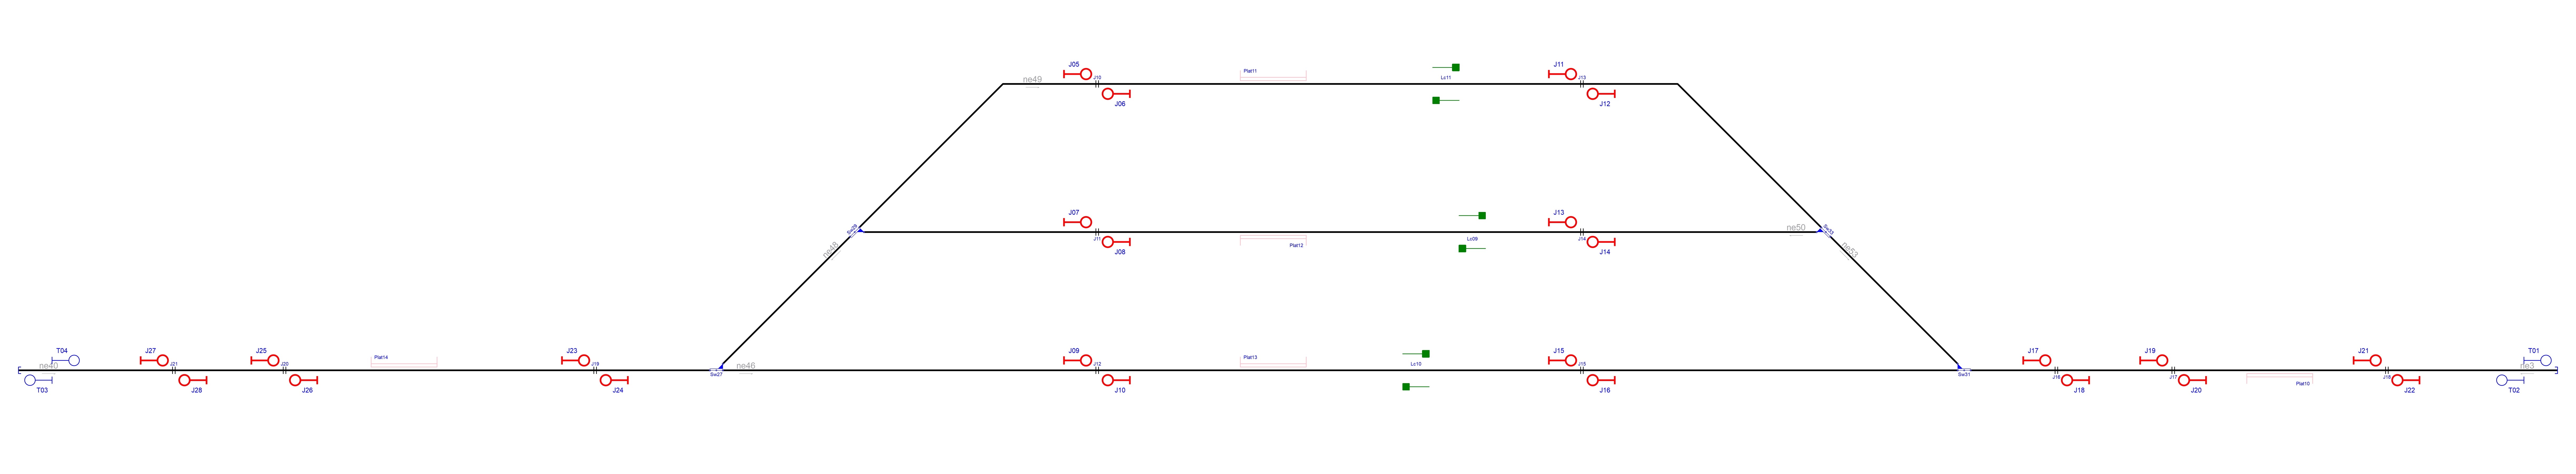
\includegraphics[width=1\textwidth]{resultados-obtenidos/ejemplo9/images/9_step2.png}
	\centering\caption{Señalamiento generado por el RNA para proteger las junturas.}
	\label{fig:EJ9_4}
\end{figure}

Al generar el señalamiento para proteger la infraestructura, tal como se explicó en la Sección \ref{sec:horizontal}, el Algoritmo \ref{alg:horizontal} simplificará las señales entre dos elementos ferroviarios si no existe espacio suficiente entre ellos, tal como sucede con los elementos Lc09 y Plat12. El señalamiento generado para proteger las plataformas y los cruces de vía se ilustra en rojo en la Figura \ref{fig:EJ9_5}. Las señales generadas para proteger las plataformas no fueron generadas, al encontrarse próximas a las señales de protección de junturas, por lo que el RNA decidió no superponer ambas señales. Mientras que las señales que protegen los cruces de vía son las señales X29 a X34.

\begin{figure}[H]
	\centering
	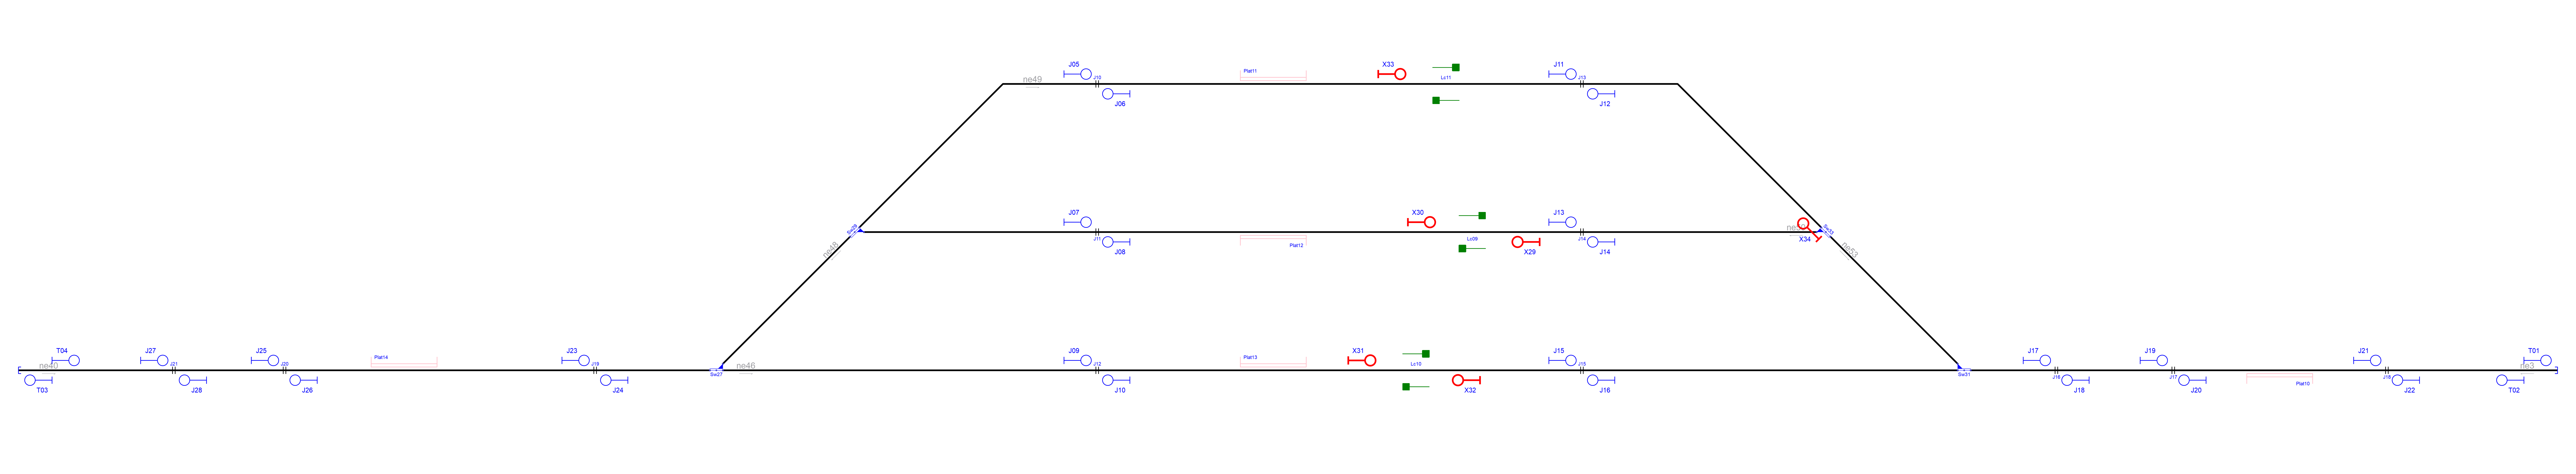
\includegraphics[width=1\textwidth]{resultados-obtenidos/ejemplo9/images/9_step3.png}
	\centering\caption{Señalamiento generado por el RNA para proteger plataformas y cruces de vía.}
	\label{fig:EJ9_5}
\end{figure}

'C35', 'S36', 'H37', 'H38', 'C39', 'B40', 'C41', 'S42', 'H43', 'H44', 'C45', 'B46'

El RNA generó las señales S36 , C35, H36 y H38 para proteger el cambio de vías Sw27; las señales S42, C41, H43 y H44 para proteger el cambio de vías Sw31; las señales C39 y B46 para proteger el cambio de vías Sw29 y la señal C45 para proteger el cambio de vías Sw33. Las señales mencionadas se encuentran resaltadas en rojo en la Figura \ref{fig:EJ9_6}.

\begin{figure}[H]
	\centering
	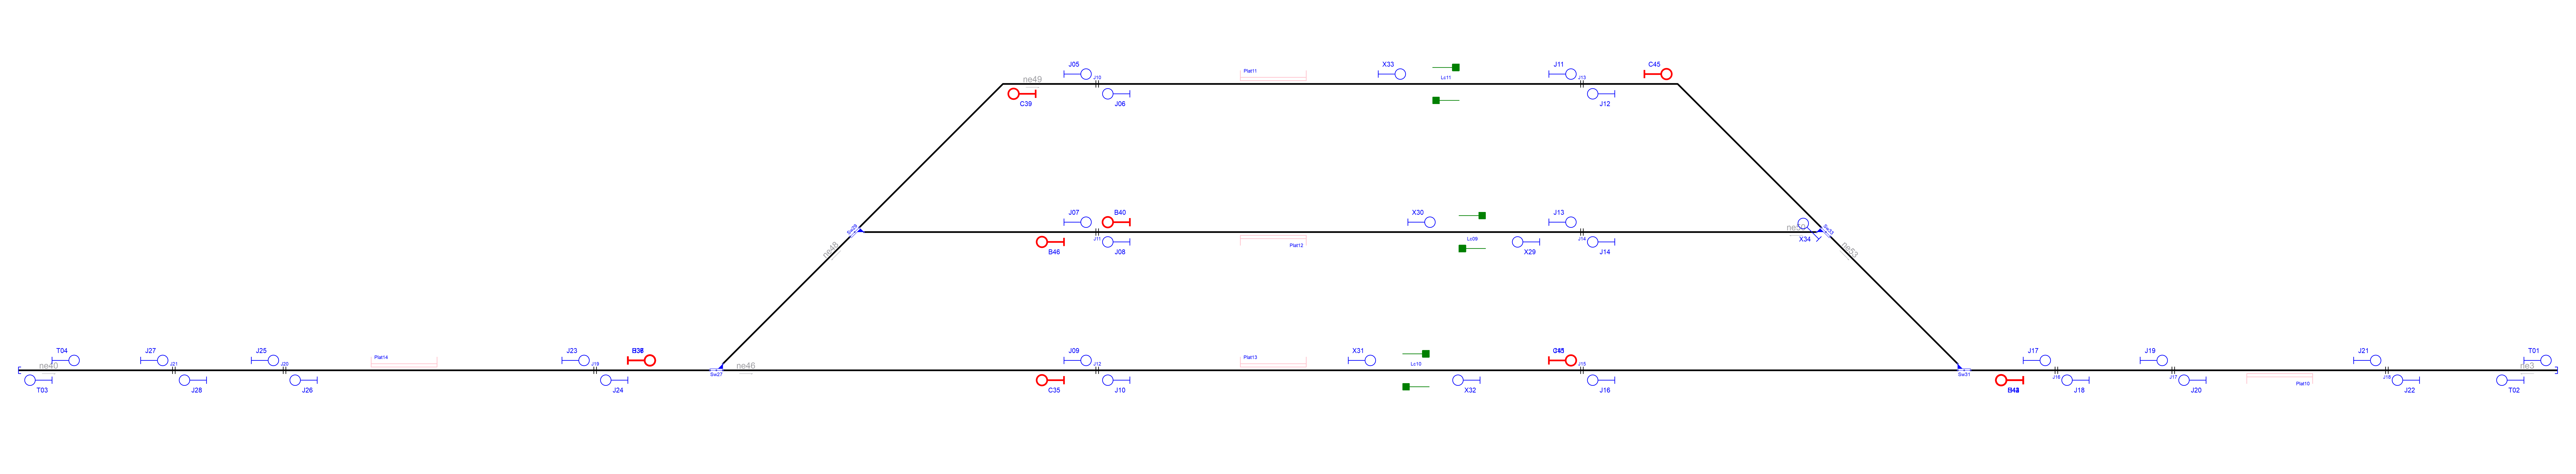
\includegraphics[width=1\textwidth]{resultados-obtenidos/ejemplo9/images/9_step4.png}
	\centering\caption{Señalamiento generado por el RNA para proteger los cambios de vías.}
	\label{fig:EJ9_6}
\end{figure}

Una vez obtenido todo el señalamiento, el RNA procede a simplificar las señales redundantes, repetidas o cuyas funciones o ubicaciones se superponen entre sí. El proceso de simplificación de señales fue explicado en la Sección \ref{sec:simplificacion}. El Algoritmo \ref{alg:vertical} de herencia vertical fue aplicado en las señales B entre los cambios de vías Sw31 y Sw33, desplazando las señales hasta convertirlas en las señales H43 y H respectivamente. Análogamente, entre los cambios de vías Sw27 y Sw29 se convirtieron en las señales H37 y H38 respectivamente.

Las señales simplificadas al aplicar el Algoritmo \ref{alg:horizontal} de herencia horizontal son: J22, J28, J27, C39, J08, C35, C45, X34, X30, X29, J15, X32, J19, J20, J18, J23, H37, H38, B40, H43 y H44. Las señales J23, H37 y H38 fueron eliminadas por su cercanía con la señal S36, con la cual comparten dirección y sentido. Lo mismo ocurre entre el par de señales H43/H44 y la señal S42; además de varios otros casos de simplificaciones simples. En todos los casos, se aplicó el Algoritmo \ref{alg:horizontal}, diseñado para agrupar objetos cercanos como un único objeto, generando el señalamiento acorde a los elementos contenidos en cada extremo del nuevo elemento contenedor.

Finalmente, las señales son simplificadas aplicando el Algoritmo \ref{alg:reduction} de eliminación por prioridad de señales. El resultado de este proceso es detallado en el Código \ref{lst:EJ9_3}.

\begin{lstlisting}[language = {}, caption = Reducción de señalamiento por prioridad de señales, label = {lst:EJ9_3}]
	Reducing redundant signals
	removing J22 for T02
	removing J28 for T03
	removing J27 for T04
	removing C39 for J06
	removing J08 for B40
	removing C35 for J10
	removing C45 for J11
	removing X34 for J12
	removing X30 for J13
	removing X29 for J14
	removing J15 for C41
	removing X32 for J16
	removing J19 for J17
	removing J20 for J18
	removing J18 for S42
	removing J23 for S36
	removing H37 for S36
	removing H38 for S36
	removing B40 for B46
	removing H43 for S42
	removing H44 for S42
\end{lstlisting}

	El resultado de la simplificación del señalamiento se ilustra en la Figura \ref{fig:EJ9_7}.
	
	\begin{figure}[H]
		\centering
		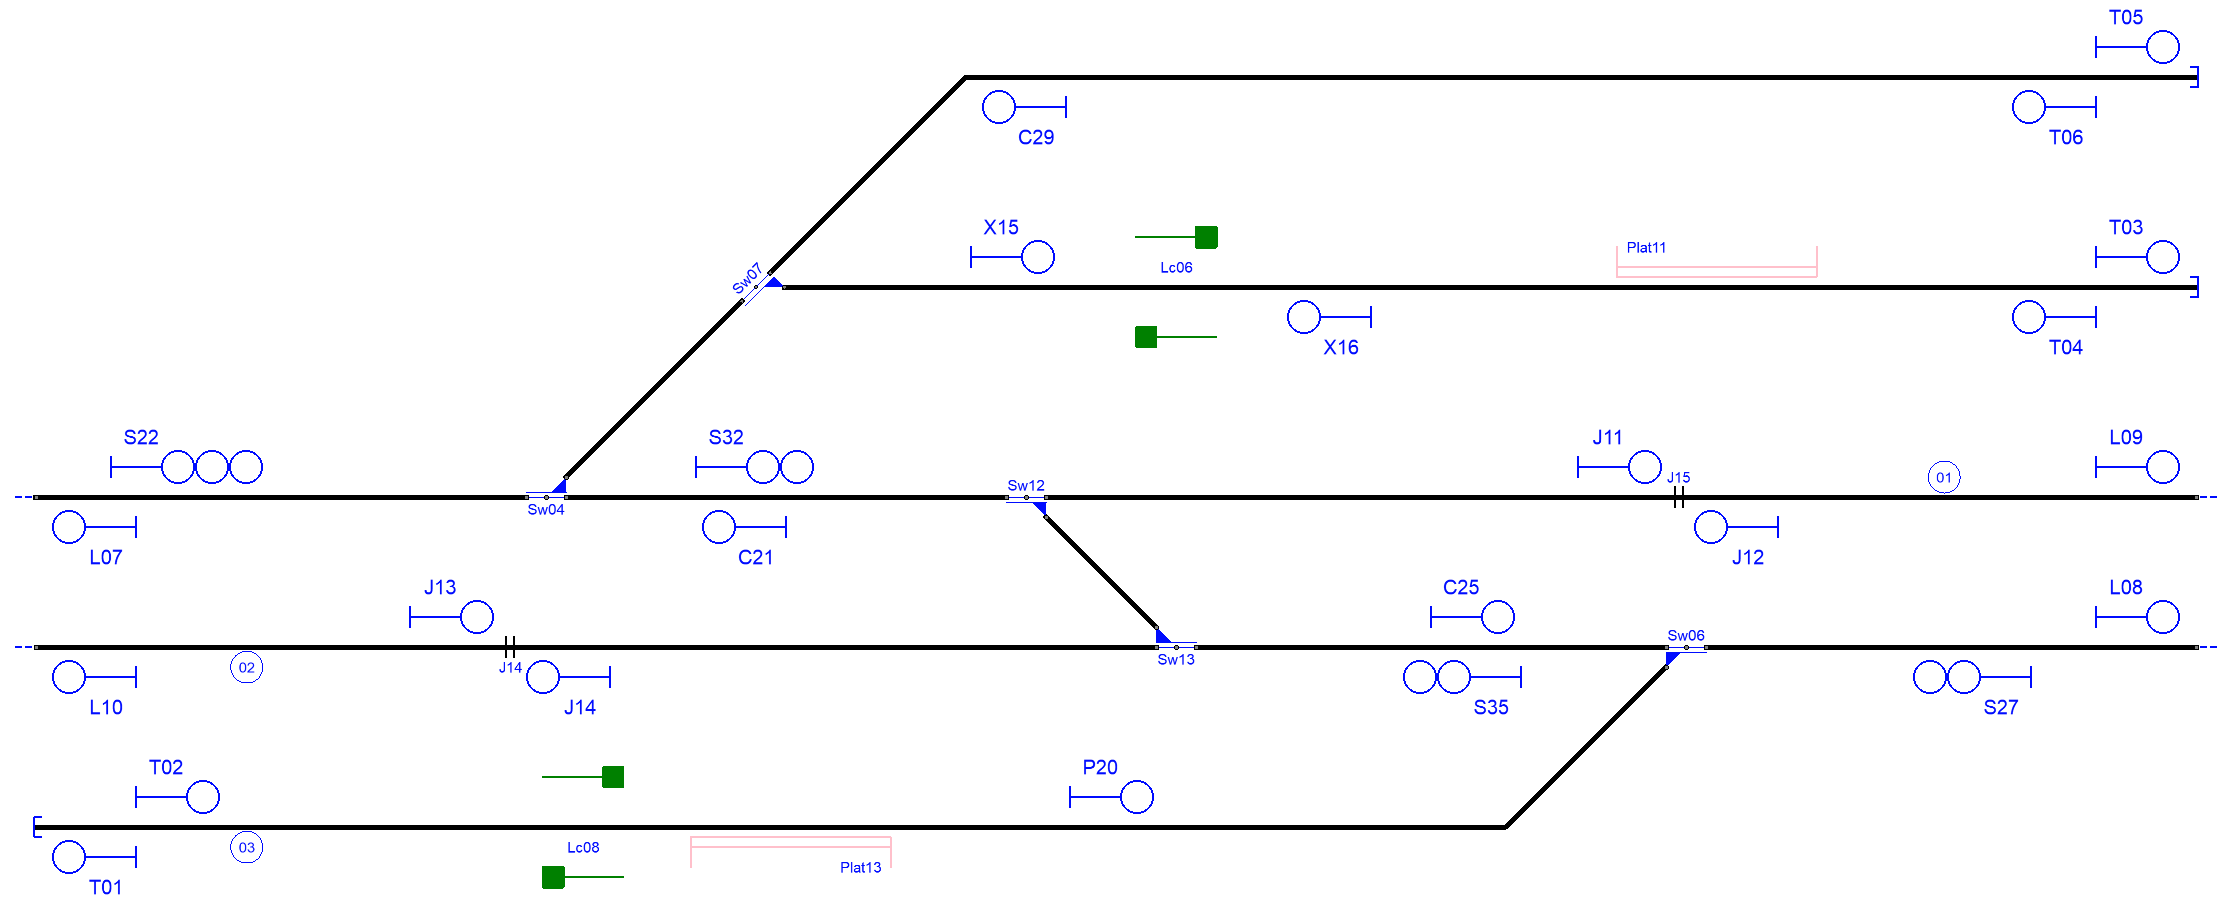
\includegraphics[width=1\textwidth]{resultados-obtenidos/ejemplo1/images/1_RNA.png}
		\centering\caption{Señalamiento generado y simplificado por el RNA.}
		\label{fig:EJ9_7}
	\end{figure}
	
	Al finalizar la generación del señalamiento, el RNA debe detectar todas las posibles rutas admitidas por la red para crear la tabla de enclavamientos. El RNA exporta los resultados del análisis en los siguientes cuatro documentos: Infrastructure.RNA (Apéndice \ref{sec:infrastructureRNA}), SafePoint.RNA (Apéndice \ref{sec:safePointsRNA}), Signalling.RNA (Apéndice \ref{sec:signallingRNA}) y Routes.RNA (Apéndice \ref{sec:routesRNA}).